\documentclass{article}

% if you need to pass options to natbib, use, e.g.:
% \PassOptionsToPackage{numbers, compress}{natbib}
% before loading nips_2018

% ready for submission
%\usepackage{nips_2018}

% to compile a preprint version, e.g., for submission to arXiv, add
% add the [preprint] option:
\usepackage[preprint]{nips_2018}

% to compile a camera-ready version, add the [final] option, e.g.:
%\usepackage[final]{nips_2018}

% to avoid loading the natbib package, add option nonatbib:
% \usepackage[nonatbib]{nips_2018}

\usepackage[utf8]{inputenc} % allow utf-8 input
\usepackage[T1]{fontenc}    % use 8-bit T1 fonts
\usepackage{hyperref}       % hyperlinks
\usepackage{url}            % simple URL typesetting
\usepackage{booktabs}       % professional-quality tables
\usepackage{amsfonts}       % blackboard math symbols
\usepackage{nicefrac}       % compact symbols for 1/2, etc.
\usepackage{microtype}      % microtypography
\usepackage[super]{nth}     % JK: for 1st-ing and 2nd-ing

\usepackage{graphicx}       % added by seth - image support
\graphicspath{ {./images/} }
\usepackage{wrapfig}        % added by seth for placing images in-line with text

\usepackage{hyperref}
\hypersetup{
    colorlinks=true,
    linkcolor=blue,
    filecolor=magenta,
    urlcolor=blue,
}
 
\urlstyle{same}
\title{%
  Kung Faux Pandas \\
  \large Simplifying privacy protection
  }

\author{
  James King, Seth Russell, Tellen D. Bennett, Debashis Ghosh\\
  Data Science to Patient Value (D2V), School of Medicine\\
  University of Colorado Anschutz Medical Campus, Aurora, CO\\
  \texttt{\{james.king, seth.russell, tell.bennett, debashis.ghosh\}@ucdenver.edu}}

\date{May 2018}

\begin{document}

% Advice from Tell:  articulate the problem with evidence (i.e. papers)
%   Enable reproducibility - patient value, make process of replication easier
%   Time saving
%   legal risk (carrying data in laptops, etc)
%   Multiple comparison?
%   Educational data sets
%  Definition of :reproducibility 
%       reproducibilty - everything same - code, data, result
%       replicability - code same, new data, same result find Peng & Leek reference (also look at blog)
%   unit testing...
%   Proof of privacy guarantees?

\maketitle

\begin{abstract}
There are many barriers to data access and data sharing, especially in the domain of machine learning on health care data. Legal constraints such as HIPAA protect patient privacy but slow access to data and limit reproducibility. We provide a description of an end-to-end system called \emph{Kung Faux Pandas} for easily generating de-identified or synthetic data which is statistically similar to real data but lacks sensitive information. This system focuses on data synthesis and de-identification narrowed to a specific research question to allow for self-service data access without the complexities required to generate an entire population of data that is not needed for a given research project. Kung Faux Pandas is an open source publicly available\footnote{\url{https://github.com/CUD2V/kungfauxpandas}} system that lowers barriers to HIPAA- and GDPR-compliant data sharing for enabling reproducibility and other purposes.
\end{abstract}

\section{Introduction}

Independent reproduction and replication of results are critical components of scientific inquiry. Barriers to data access and sharing are the most important impediments to reproducibility in machine learning (ML) research. Health care research has unique challenges because of necessary personal data privacy protections.

Several methods exist to de-identify (remove key identifiers, group individuals, and related anonymization techniques \cite{hippapro}) and synthesize data (create data through algorithmic means, population level statistics, randomization, ideally with preservation of multivariable relationships between records \cite{walonoski_synthea_2018, patki_synthetic_2016, choi_generating_2017}). However, no pipeline currently exists with which ML investigators can routinely \emph{anonymize} or \emph{synthesize} data to facilitate access and sharing. This work addresses that gap.

We have created an open source software library called \emph{Kung Faux Pandas (KFP)} which allows for the modular combination of established privacy protection methods with the popular Python Pandas data science library\cite{mckinney-proc-scipy-2010}. KFP also provides a Structured Query Language (SQL) interface which enables users to query a database and receive a data set without personal information through either anonymization or synthetic data generation.

\section{Background}

Recent work has clarified the definition and importance of reproducibility and a closely related concept, replicability. Leek and Peng have defined reproducibility as the "ability to recompute data analytic results given an observed dataset and knowledge of the data analysis pipeline," and replicability as "the chance that an independent experiment targeting the same scientific question will produce a consistent result."\cite{leek_opinion_2015,peng_reproducible_2006} There is broad agreement that an independent experiment with confirmatory results is the strongest support of any experiment. One early influential paper on the topic of reproducibility in scientific computing lists the key factors in reproducibility as available data, input parameters, documentation, software code, and an environment capable of running the provided software code. These items are difficult to convey in a traditional research paper \cite{schwab_making_2000}.

In the context of ML, sufficient detail is required such that an independent investigator could create the same hardware and software configuration, data used for all experiments, source code, documentation on data and how to run/configure software, and tests that verify the software runs correctly. Once a result can be reproduced, new researchers can then build upon the methods, gather new data for testing/validation, or discover alternative methods to replicate a result.

Many domains in which ML investigators work have legal barriers that make it difficult to enable independent verification of ML models due to data access issues. As an example, in the health care domain in the US, a key law governing health data is the Health Insurance Portability and Accountability Act (HIPAA). HIPAA is backed by significant civil penalties, specifics about data security, and what can be done with protected health information \cite{hippaviol}. While there are other domain specific data privacy laws, there are also some broad rules such as the European Union's General Data Protection Regulation (GDPR). The GDPR puts in place new rules about data ownership and control in an attempt to give individuals more control over their information.

Early examples of re-identification attacks \cite{sweeney_2002} have have created apprehension on the part of businesses and legal experts in data sharing \cite{ohm_broken_2009}. More recently, research in the data sharing/privacy protection space has focused more on synthesis techniques such as in the case of the Synthea system \cite{walonoski_synthea_2018}. Current solutions are not without their drawbacks however as many require significant configuration of metadata before they can generate data or they attempt to solve the entire solution space and consequently are very slow to run.

\section{System Details}

One way around the difficulties of source data access is to separate the dependency between data and analysis in such a way that analysis can be performed without the analyst having access to the source data. Such a process can be possible if a sufficiently detailed description of the sensitive data is provided. Appropriate models can be developed and initially validated before either being handed off to a data custodian who then runs the processes on protected data and returns the results to the researcher or access to the protected data has been granted directly to the researcher. Solutions of this form have been possible for some time, but are awkward in practice because activities such as data cleaning, exploration, and model building are interactive and iterative processes that require more than just descriptions of data.

KFP addresses the issue of data access by generating data that is similar to the real data but does not itself contain any sensitive data. We collectively refer to de-identified data and synthetic data as \emph{faux-data}. We use the term faux as it is used in the fashion sense of the word: the use of man made materials that look and feel like real leather, fur, etc., but without the problematic derivation from live animals and reliance upon limited resources. Faux-data can be analyzed, cleaned, modeled etc. as if it were the actual source data. KFP provides a standard mechanism for wrapping a privacy protection method into a plug-in which integrates the method with the Pandas DataFrame model. Two of these plug-ins are provided with full documentation for creating other plug-ins.

As the data generated through KFP has no protected component, it can be shared along with code or methods to improve reproducibility as well as aid in replicability. To further the aim of reproducibility we have provided our code and a sample of a randomly generated dataset for testing purposes through our GitHub repository in a range of formats: Python environment files (conda and pip) to allow others to start with the same software libraries and specific versions that we used, a Docker container with code and sample data installed and already configured, and all source code along with version history so others can follow our development process.

KFP focuses on generating faux-data narrowed to a specific subset that a researcher is interested in rather than attempting to generate an entire population of data such as an entire EHR. By focusing on just the data needed, performance is improved, the need for extensive modeling or metadata configuration is reduced, and the amount of faux-data generated and stored is minimized. Although the plugable methods included for faux-data generation have been shown to effectively replace source data for analysis, KFP facilitates a more through process that includes an initial exploration with faux-data followed by a repetition of methods on original source data through query logging and thereby aiding in replication.

\subsection{System Architecture}

Ideally a ML investigator should develop, test, and validate models using all available data. This is most easily accomplished when they have unfettered access to all data in the problem domain they are working in. The novel architecture of KFP is that direct data access is provided through an intermediary that can synthesize data on-demand.

\begin{figure}[ht]
  \centering
  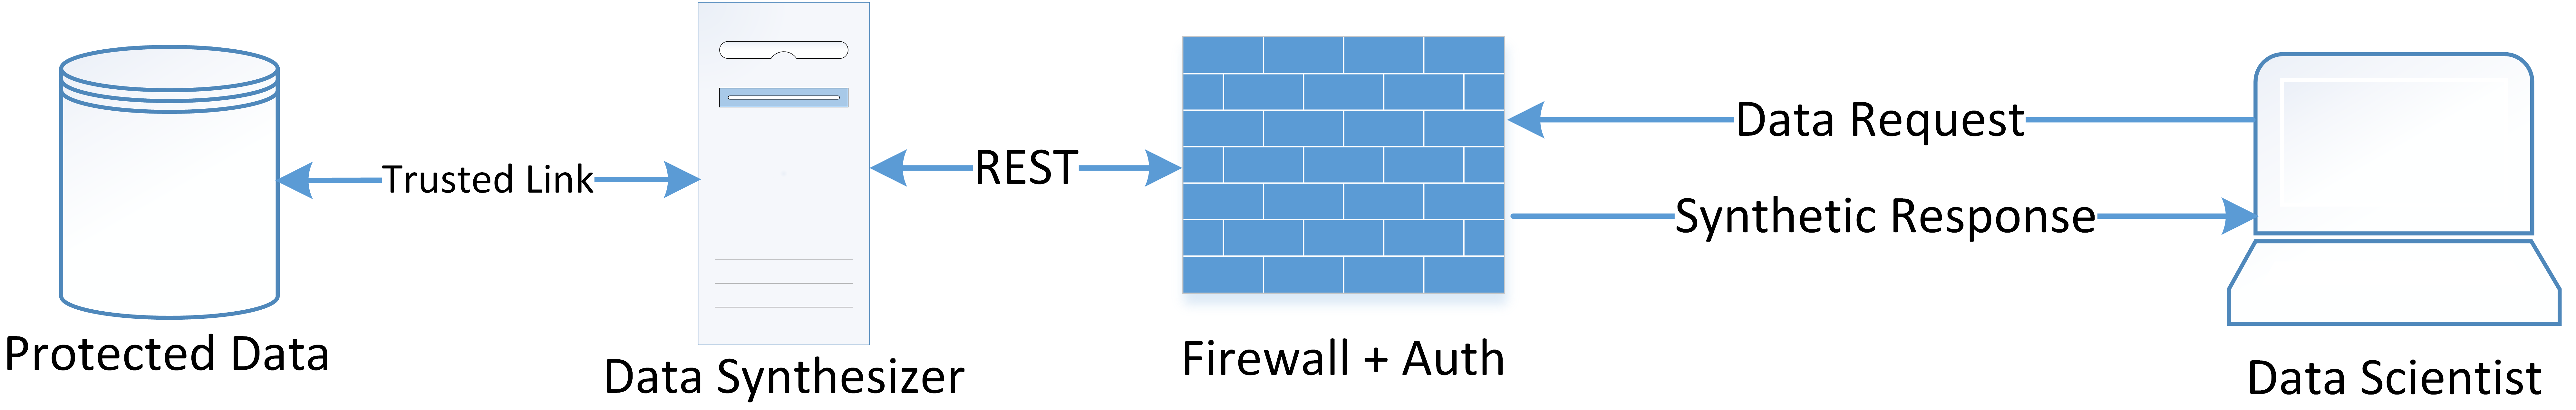
\includegraphics[width=120mm]{prototype_architecture}
  \caption{System Architecture.}
  \label{fig:architecture}
\end{figure}\begin{figure}[ht]
  \centering
  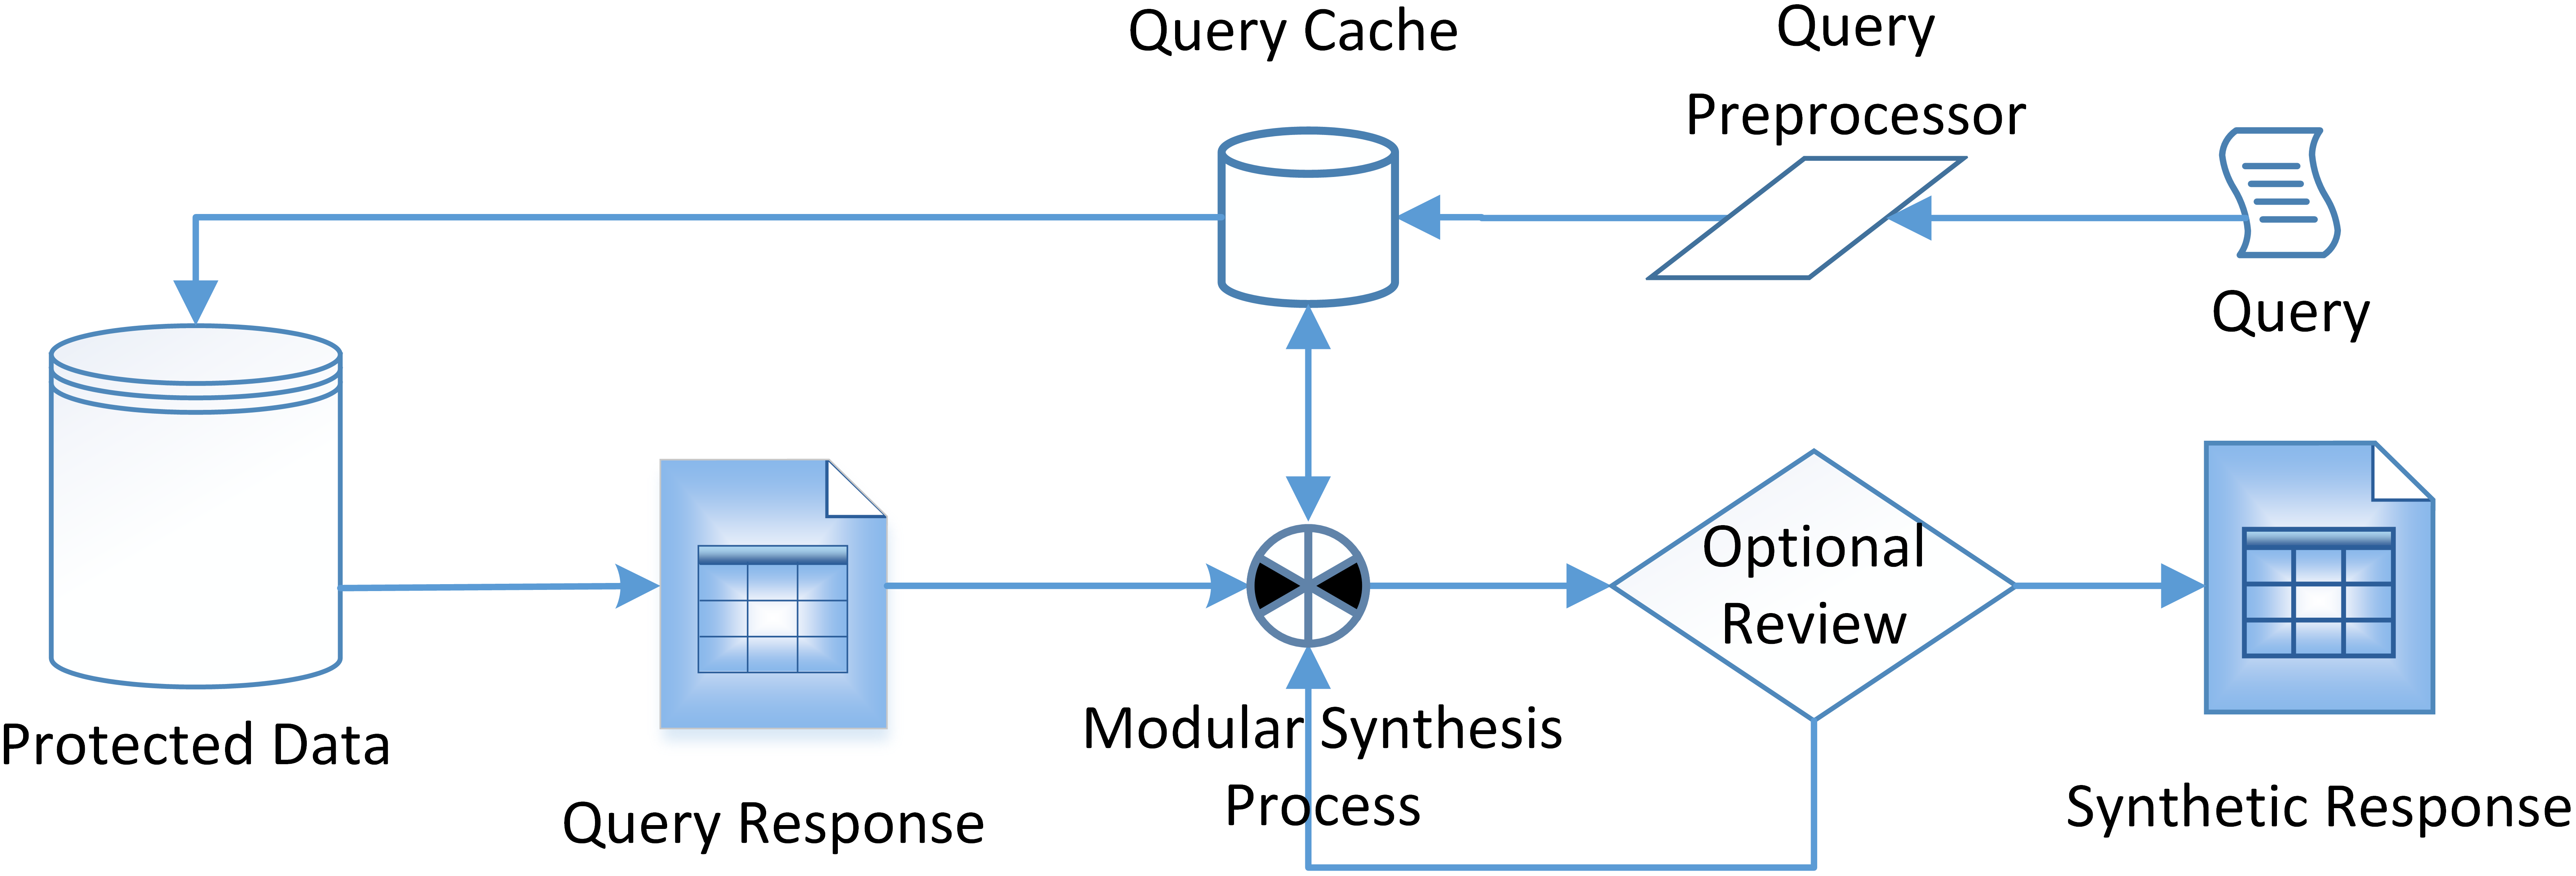
\includegraphics[width=100mm]{data_synthesis_process}
  \caption{Data synthesis process.}
  \label{fig:synthesis_process}
\end{figure}

Figure~\ref{fig:synthesis_process} shows the automated faux-data request/response process. All queries submitted to the system are first pre-processed to remove clauses such as "ORDER BY" which are made ineffective by the synthesis process. All queries are logged for later analysis and results cached to optionally improve synthesis performance for repeated queries. Next the processed query is executed against the protected data set and results are passed into the modular synthesis process. While the current
\begin{wrapfigure}[15]{r}{0.5\textwidth}%optionally place [15] after {wrapfigure} to control how many lines to wrap around figure
  \centering
  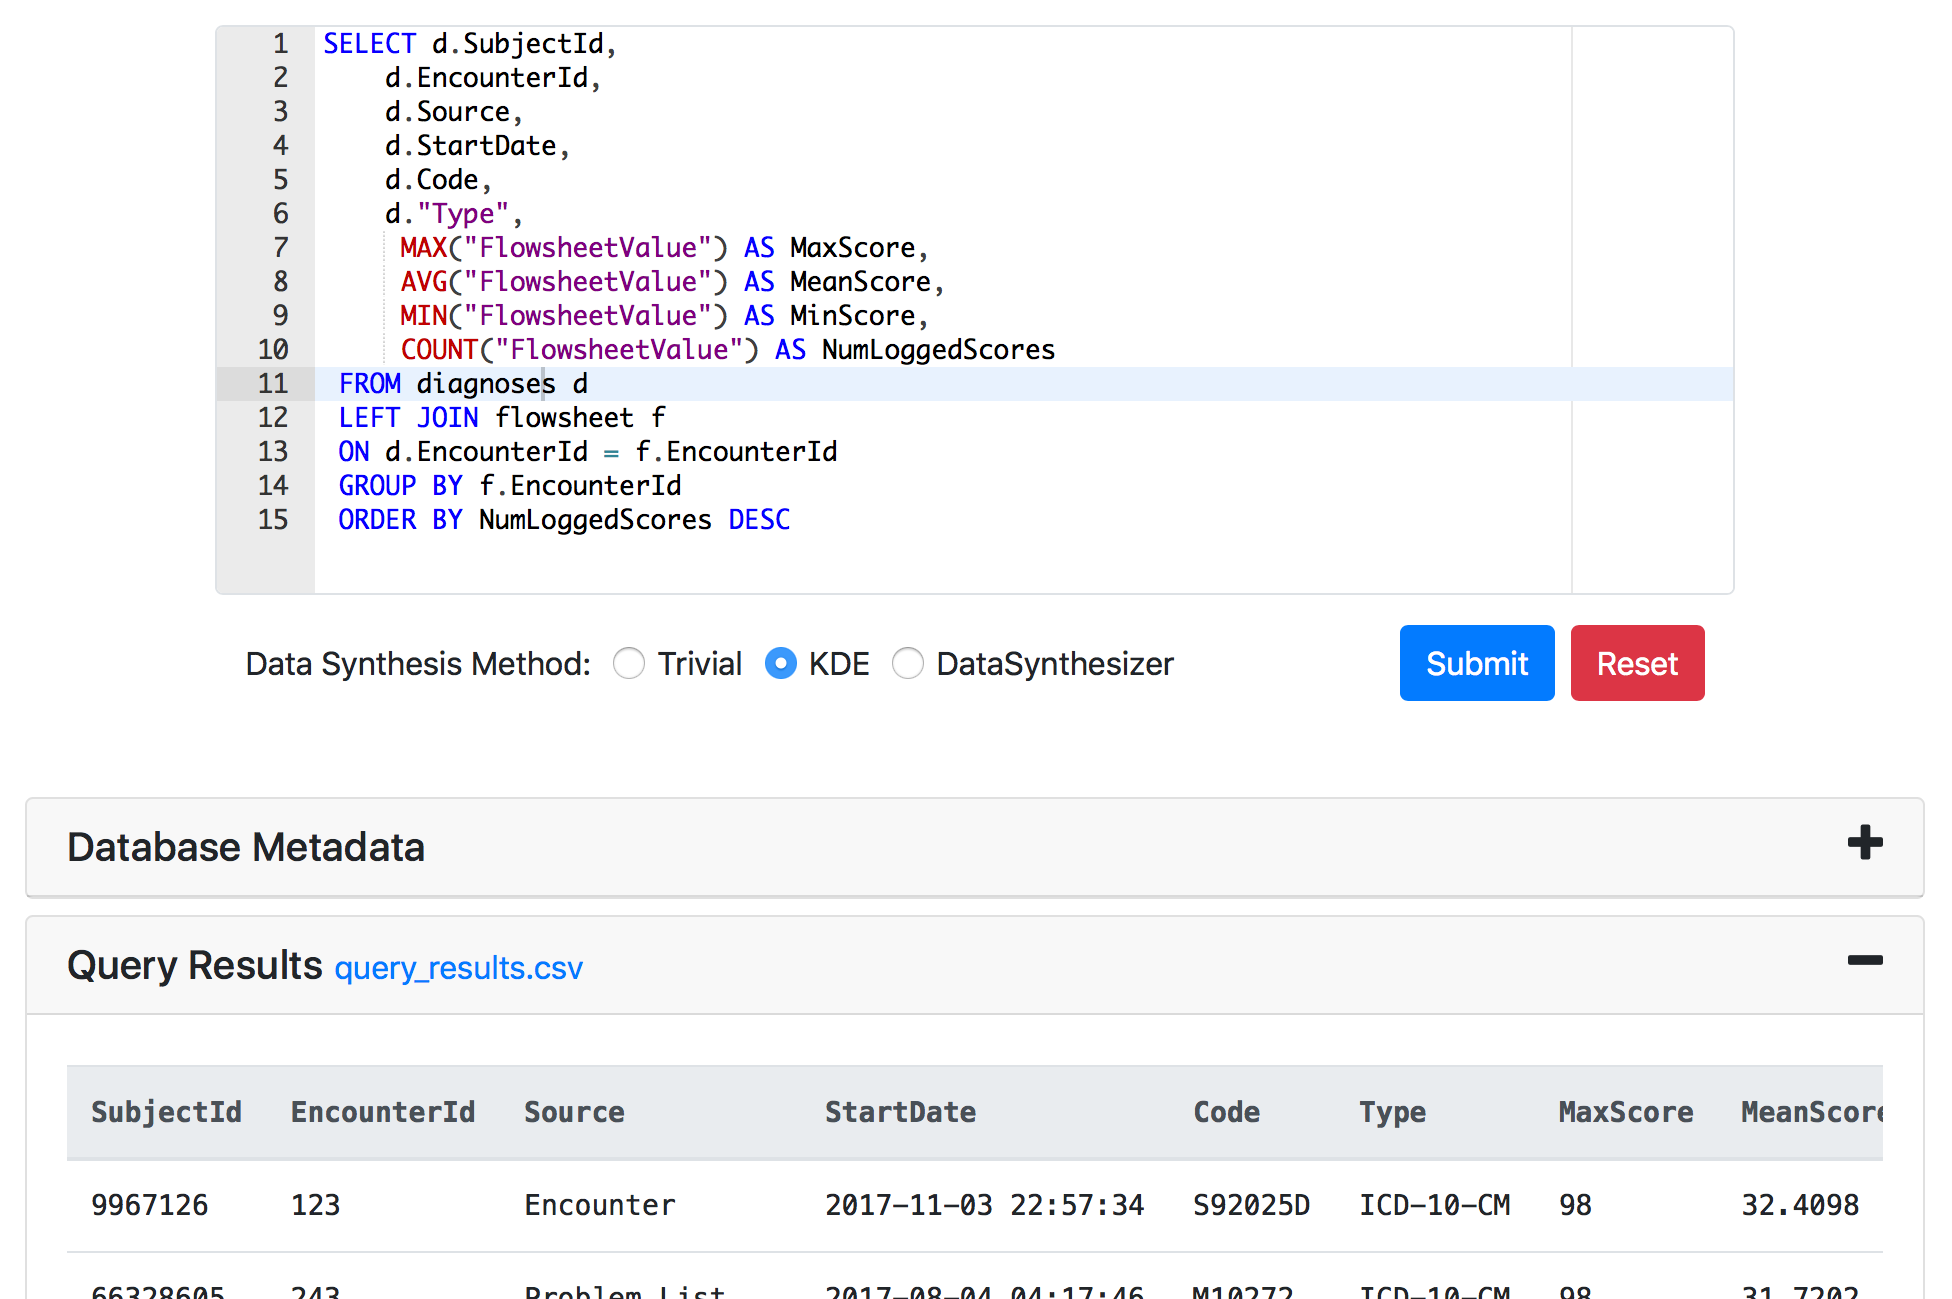
\includegraphics[width=0.5\textwidth]{ui_screenshot3}
  \caption{User Interface.}
  \label{fig:ui}
\end{wrapfigure}
implementation only utilizes a couple of synthesis methods, ML developers or data owners can insert their own custom method or modify existing methods. Previously removed "ORDER BY" clauses are re-applied to the faux-data before results are returned to the user. Finally, although not implemented in this version of KFP, synthetic results could be held back until reviewed and approved for release by the data owner.

KFP provides multiple methods by which a ML developer can access on-demand faux-data. As shown in Figure~\ref{fig:ui}, a single page web application (SPA) allows for users to directly enter SQL queries, submit them to the connected database, and receive faux-data according to the selected generation method. Data can either be viewed directly in browser or downloaded in csv format for use in a ML process. Alternatively, a Hypertext Transfer Protocol (HTTP) Representational State Transfer (REST) service \cite{w3c_working_group_webservices}, utilized by the SPA, allows for cross language compatible requesting and receiving of faux-data, again via SQL query. In order to facilitate querying and understanding of the data model, the database metadata is presented to the user in a collapsible section. Lastly, for Python based software or languages with an interface to Python, the kungfauxpandas.py file and associated classes can be imported and called natively.

\subsection{Included Synthesis Methods}

KFP provides a framework by which any number of methods for data privacy can be carried out. For demonstration purposes we have implemented two plugins that use different techniques for data synthesis. The kernel density estimator from scipy.stats.gaussian\_kde uses the method developed by Silverman \cite{silverman_density_1986} which handles inter-related ordinal and ratio data yet runs quickly on standard consumer level hardware. The DataSynthesizer method, created by Ping et al. \cite{ping17datasynthesizer} is built on differential privacy mechanisms and has multiple internal methods for data generation ranging from random generation based on data type to Bayesian modeling of inter-relationships among columns of data. In DataSynthesizer, the authors show that the synthetic data generated preserves privacy while still being useful enough for actual data analysis (see also \cite{howe_synthetic_2017}).

\section{Discussion}

KFP provides a unique contribution to the space of reproducible ML. Through providing ad-hoc faux-data, ML researchers can have lower barriers to accessing private data as well as reduced barriers to sharing faux-data derived from private data. However, there are several areas that could be researched further: improved code sharing, addressing institutional specific privacy issues, and evaluation of this system in a ML workflow.

While we have provided software code and a description of our methods, we believe that ML reproducibility should go beyond just making source code available. Peng recommends that code should be made available "in a durable non-proprietary format" \cite{peng_reproducible_2011}. This is a level of code sharing rarely achieved in ML research. Currently there is no standard long term format that works for all computational environments. For the Python ecosystem however, the standard for sharing code is via a package on Python Package Index (PyPI). We intend to continue this research to make KFP available as a Python package.

Another area that is open for further research is that of domain and institution specific data privacy needs. In the field of education, statistical methods for calculating sample size based on probability of detecting a specific effect size are commonly used \cite{naep_2009} as the key method for privacy protection. However, it is not clear that these methods are appropriate for use in ML in general or domains other than education. KFP could be modified to return no results if a minimum threshold is not met or, alternatively, data boosting techniques in combination with data synthesis could be used based on the risk profile of the data owner(s).

The last area recommended for further research is to deploy and observe the use of KFP in an active ML environment where researchers are working with sensitive datasets. A key limitation that may be identified is that of performance characteristics, particularly in a multi-user setting against a large relational database store. Additionally, actual reviews by security and compliance groups or institutional review boards may uncover additional requirements to reduce risk of data exposure that could require significant rework or further study.

\section{Conclusion}

KFP removes barriers to data access and data sharing via self-service faux-data generation. Users of KFP do not need to have access to a protected dataset nor does a human have to be involved in translating researchers data needs into a non-protected dataset. This self-service data can be differentially private or meet other privacy needs based on plugin capabilities. With faux-data, researchers can publicly share data upon which their research relies without organizational fear of privacy breaches. KFP also facilitates a process by which evaluation, analysis, or model building is first performed with faux-data followed by repetition upon private data. 

Finally, instead of taking the computational and labor intensive step of full EHR de-identification or synthesis, KFP takes the smaller and more easily implemented step of just-in-time data de-identification or synthesis. We surmise that this tool will improve data exploration and reduce dependency on complex processes required for data access. The result of this system will be improved reproducibility in ML.

\bibliographystyle{unsrt}

\bibliography{bib}

\end{document}